\section{Fundamentals}
\label{sec:fundamentals}

\subsection{Raycasting}

Ray casting is primarily an imaging technique and was first described by Scott Roth in 1982 as an effective method of rendering CSG (Constructive Solid Geometry) objects. Although ray casting may be used for different purposes in various dimensions, we will focus on generating a two dimensional image from a three dimensional scene. The basic principle therefore is shown in figure \ref{fig:raycasting}. 

\begin{figure}
\centering
\includegraphics[width=0.6\textwidth]{raycasting}
\caption{Principle of ray casting.}
\label{fig:raycasting}
\end{figure}

Generating an image of a three dimensional scene of objects is done by sending rays from a defined eye point through the image plane into the scene. The image plain resembles the two dimensional output image which should be generated. Each output pixel is transformed into a three dimensional position on the image plane which is passed through by one ray originating from the eye point. The eye point itself is usually positioned centered before the image plane to achieve a perspective view of the scene. Each ray is then guided through the three dimensional space containing the scene objects trying to find an intersection. In the case an object is hit, a color value is calculated for the intersection point on the object (using e.g. materials parameters or textures of the surface). The pixel on the image plane, through which the ray was shot initially, is then set to this color.

Ray casting is different from the wide-spread rasterization used for most 3D applications and computer games today as it approaches from the image side instead of the objects, the scene is composed of. Rasterization takes all the objects placed in the scene (which have to be composed of primitive shapes, mostly triangles) and transforms them from three dimensional space to the two dimensional space of the output image where each object is then rasterized onto the pixels of the output image.

Apart a lot of technical differences, both methods also differ in complexity. Mark Kilgard describes the complexity of rasterization with $\mathcal{O}(b * m)$ whereas an accelerated ray tracing implementation (e.g. using a favorable data structure) achieves $\mathcal{O}(log b * p)$, where $b$ is the number of objects in the scene, $m$ is the average number of pixels per object and $p$ is the number of pixels in the scene \cite[p.48]{ray_casting_presentation}. The Enlight proposal additionally points out, that the size of computer screens increased far slower over the past decades than the size of computer memory, computational power and the size of industrial CAD (Computer-aided design) and CAM (Computer-aided manufacturing) models \cite{enlight_proposal}. Therefore, ray casting might be beneficial when used to render large scenes compost of huge amounts of triangles.


\subsection{Regular grids}
\label{sec:regular_grids}

Regular grids are a type of data structure frequently used in ray casting/tracing to accelerate the traversal of rays through the scenes. Alternative approaches are often tree based such as kd trees, octrees, binary space partitioning (BSP) or bounding volume hierarchy (BVH). Each of these techniques has its own strengths and weaknesses depending on the scene and application. However, especially kd trees and grids (and multilevel grids) have been primarily focused in recent work about interactive ray casting/tracing \cite[ch.1]{packet_caster}. While kd trees usually perform amazingly well on static scenes, dynamic or animated objects still present a challenge as the used data structure has to be rebuilt after every scene change, which can take up to several seconds for larger sets of geometries \cite[ch.1]{packet_caster}. Regular grids are simpler structures for partitioning space and accelerating ray casting. They can be created quicker than a (balanced) tree, thus allowing more frequent scene changes. Nevertheless, kd trees may be up to a magnitude faster when it comes to the actual ray traversal \cite[ch.1]{packet_caster}. As Enlight focuses on visualizing dynamic scenes (for subtractive manufacturing) allowing at least ten subtraction volumes to be added to the scene per second, regular grids appear promising for being used in this case.

Building a regular grid data structure is simple. Initially, a bounding box is created around the scene. This box is then divided into equally sized cubes (which may force the box to be enlarged a bit to fit a whole number of cubes in each dimension) which are called cells. For each object (triangle) of the scene all spanned cells are calculated and the cells store a reference to the triangle.

\begin{figure}
\centering
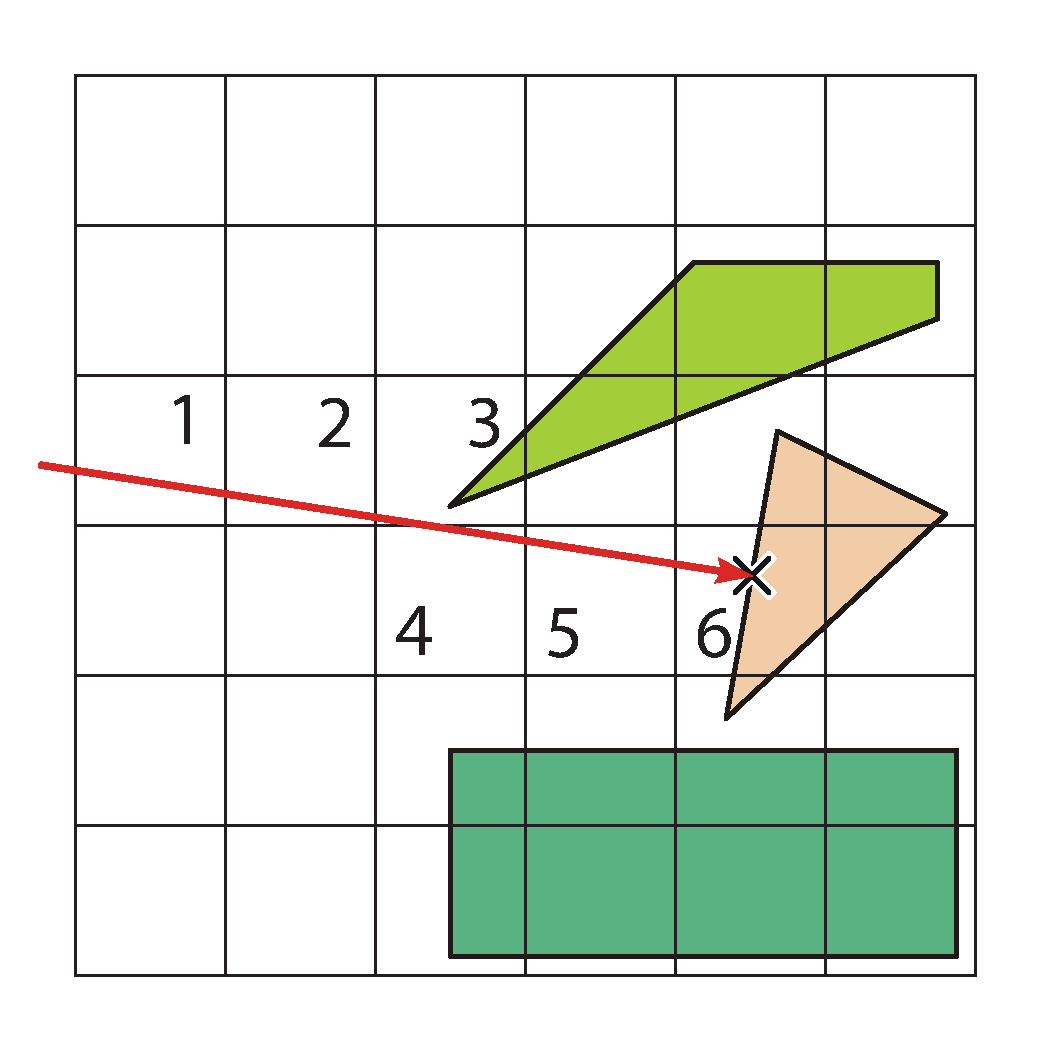
\includegraphics[width=0.4\textwidth]{cell_traverser}
\caption{Traversing the cells of the grid using a DDA variant until an intersection has been found.}
\label{fig:cell_traverser}
\end{figure}

During ray casting, the rays have to traverse the cells of the grid in order to find potential geometry they might intersect with (cf. figure \ref{fig:cell_traverser}). A fast algorithm for traversing regular grids using a single ray is given by John Amanatides and Andrew Woo \cite{3DDDA}. Their algorithm is a slight modification of the DDA (digital differential analyzer) which is used for the rasterization of lines. As finding the pixels (squares inside a regular 2D grid) which are covered by a line is actually the same problem as finding the voxels hit by a ray, this adapted 3D DDA algorithm can be used for efficient traversal of regular grids. Furthermore, as the algorithm's start point can be determined and the voxels (grid cells) are traversed incrementally, no depth sorting has to be performed across the hit cells and the traversal can be stopped on the first found intersection. Inside each cell, all triangles have to be intersected and the intersections have to be sorted by depth in order to find the hit and visible surface.


\subsection{Boolean raycasting}

Enlight focuses on subtractive manufacturing. Therefore, the scene is composed of an initial stock volume from which further volumes are subtracted (cf. goals in chapter \ref{sec:about_enlight}). This scenario can be typically found in CSG (Constructive Solid Geometry) modeling, where complex models are build from boolean combinations of simpler models. CSG models can be efficiently rendered using ray casting, by using a tree with the volumes as leaves and the boolean operations applied to them as nodes. The rays are then traversed through the scenes and have to resolve the tree on every volume entry or exit. Enlight only supports a subset of CSG by only allowing boolean subtraction from the initial stock volume. However, by inverting the stock volume (inverting the surface normals)) and defining the world space as being filled instead of empty, the problem can be even more simplified as the scene now only consists of subtraction volumes.

\begin{figure}
\centering
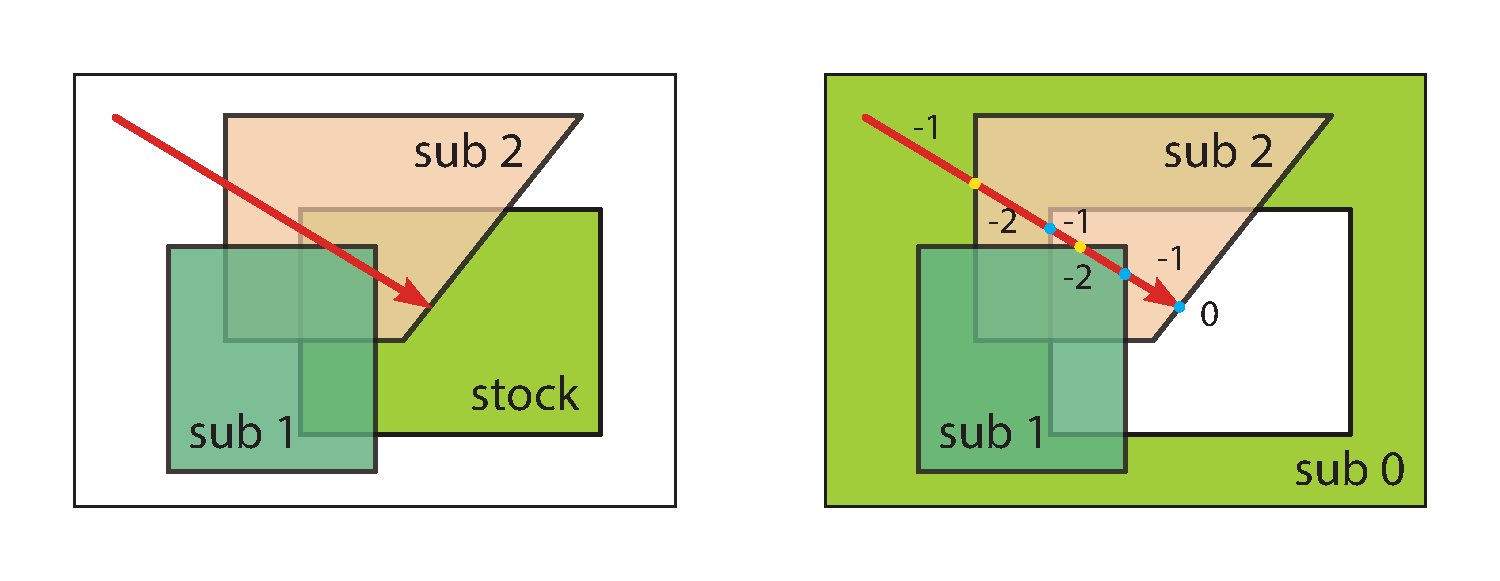
\includegraphics[width=0.8\textwidth]{boolean_casting}
\caption{Ray traversing through a scene containing one stock and two subtraction volumes. By inverting the stock (in the left figure) into a subtraction volume (invert normal vectors of surface, figure on the right), the counting algorithm is simplified. The ray starts with a counter value of minus one (inside the inverted stock volume), is decremented on every volume entry (yellow dot) and incremented on ever volume exit (blue dot). If the counter reaches the value zero, the surface has been found.}
\label{fig:boolean_casting} 
\end{figure}

The algorithm for ray casting a scene composed of subtraction volumes is illustrated in figure \ref{fig:boolean_casting}. Every ray starts outside the initial scene and maintains a counter which determines the number of subtraction volumes, the ray is inside of/has entered. As outside of the original scene is inside the inverted stock, this value is initialized with minus one (inside one volume). The ray is then traversed through the scene. On every intersection where the ray enters a volume, the counter is further decremented (the ray is now inside even more volumes). On every exit, the counter is incremented (the ray is now inside one less volume) and checked if it has become zero. A counter value of zero on a volume exit corresponds to an intersection with the surface of the resulting model.

\subsection{Packet casting}

A common technique for accelerating ray casting and tracing is to accumulate squares of adjacent rays into ray packets and traversing the packets through the scene. This technique has several advantages. Most importantly, a part of the parallelism between individual rays (which can be processed completely independent) is moved down into the traversing and intersection algorithms. As adjacent rays are likely to traverse through the same parts of the acceleration structure (e.g. the same cells of a grid) and hit the same triangles, the corresponding routines can be executed in a data parallel fashion on multiple rays. Modern CPUs and GPUs benefit from these scenarios and offer corresponding SIMD instructions (CPU) or an appropriate hardware architecture (GPU). Furthermore, coherent traversal and intersection improves caching behavior via temporal locality\footnote{Temporal locality refers to accessing the same location in memory frequently within a short time.}.

However, traversing packets through acceleration data structures such as grids is more difficult and cannot be done using the 3D DDA algorithm presented in chapter \ref{sec:regular_grids}. Fortunately, Ingo Wald et al. present an efficient solution for "Ray Tracing Animated Scenes using Coherent Grid Traversal" (which is the name of their corresponding paper) \cite{packet_caster}. Their algorithm is illustrated in figure \ref{fig:slice_traverser}.

\begin{figure}
\centering
\includegraphics[width=0.4\textwidth]{slice_traverser}
\caption{A ray packet traversing a regular grid slice by slice. The blue region is the axis aligned part of a slice (column) which is actually occupied by the packet and is determined by the corner rays of the packet. The yellow region is the blue region extended to full cell boundaries. Furthermore, the packet is always fully traversed until all rays have hit (although no intersections may be calculated for rays which have already hit.)}
\label{fig:slice_traverser} 
\end{figure}

As the ray packet may now spans multiple cells we cannot traverse cell by cell anymore. The next bigger aggregation of cells is a slice of the grid. To iterate the slices of a grid in a favorable order, the main (primary) traversal axis is determined by finding the largest component of the direction vector of one of the innermost rays of the packet (the two other axes are the secondary axes). For each slice of the grid along this main traversal axis, starting at the side of the grid where the packet enters, the four corner rays are intersected with the front and back plane of the slice. The maximum and minimum values of the intersection points along the secondary axes describe the axis aligned region of the slice which is hit by the packet (shown blue in figure \ref{fig:slice_traverser}). This region is then extended to full cell boundaries (shown yellow in figure \ref{fig:slice_traverser}). Then, all objects of the cells of this extended region have to be intersected with all rays of the packet. This routine can be easily vectorized by accumulating several rays into SIMD registers and processing the intersection tests using vector instructions (e.g. SSE, AVX). Rays which have already hit a triangle may be masked out. A further optimization to this algorithm is to cull all triangles of the selected cell region of the slice against the frustum spanned by the corner rays.


\subsection{OpenCL}

GPU hw architecture, how do kernels work? NDRange, buffers
